For the purpose of this thesis we define a \textit{tensor} $T$ \textit{of rank} $n$ as an $n$-dimensional array of complex numbers
\begin{equation}
	\label{eq:general_tensor_rank_n}
	T \in \mathbb{C}^{\chi_1\times\chi_2\times\dots\times\chi_n}, \quad \chi_i \in \{1, 2, \dots\}
\end{equation}
with entries
\begin{equation}
	T_{i_1,i_2,\dots,i_n} \in \mathbb{C}, \quad i_j \in \{1, 2, \dots, \chi_j\}.
\end{equation}
For example, a rank-0 tensor is a scalar, a rank-1 tensor is a vector, and a tensor of rank-2 is a matrix. It is convenient to use a diagrammatic notation, drawing tensors as shapes and tensor indices as lines (\textit{legs}) emerging from these shapes. As an example we draw a few simple tensors in tensor diagram notation in Figure \figref{fig:basic_tensor_diagrams}. \par
\begin{figure}[ht]
	\centering
	% Store largest image in a box
	\savebox{\largestimage}{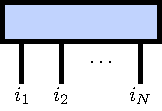
\includegraphics[scale=1]{figures/tikz/Tensor_Networks/basic_diagrams/basic_diagrams_d.pdf}}
	\subcaptionbox{\label{fig:basic_tensor_diagrams_scalar}}
	{%
		\raisebox{\dimexpr.5\ht\largestimage-.5\height}
		{%
			
\includegraphics[scale=1]{figures/tikz/Tensor_Networks/basic_diagrams/basic_diagrams_a.pdf}
		}
	}
	\quad\quad
	\subcaptionbox{\label{fig:basic_tensor_diagrams_vector}}
	{%
		\raisebox{\dimexpr.5\ht\largestimage-.5\height}
		{%
			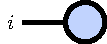
\includegraphics[scale=1]{figures/tikz/Tensor_Networks/basic_diagrams/basic_diagrams_b.pdf}
		}
	}
	\quad\quad
	\subcaptionbox{\label{fig:basic_tensor_diagrams_matrix}}
	{%
		\raisebox{\dimexpr.5\ht\largestimage-.5\height}
		{%
			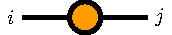
\includegraphics[scale=1]{figures/tikz/Tensor_Networks/basic_diagrams/basic_diagrams_c.pdf}
		}
	}
	\quad\quad
	\subcaptionbox{\label{fig:basic_tensor_diagrams_rank_n_tensor}}
	{%
		\usebox{\largestimage}
	}
\caption{Tensors of different ranks are shown in diagrammatic notation. (a) A scalar, (b) a vector, (c) a matrix, (d) a general tensor of rank $n$ as defined in Equation \eqref{eq:general_tensor_rank_n}.}
\label{fig:basic_tensor_diagrams}
\end{figure}
An \textit{index contraction} between two or more tensors is the linear operation that is performed by summing over a given set of indices. For example, the scalar product of two vectors $A\in\mathbb{C^\chi}$ and $B\in\mathbb{C^\chi}$,
\begin{equation}
	\label{eq:example_tensor_network_scalar_product}
	c = \sum_{\alpha=1}^{\chi}A_\alpha B_\alpha,\quad c\in\mathbb{C},
\end{equation}
and the matrix product of two matrices $A\in\mathbb{C}^{\chi_1\times\chi_2}$, $B\in\mathbb{C}^{\chi_2\times\chi_3}$,
\begin{equation}
	\label{eq:example_tensor_network_matrix_product}
	C_{ij} = \sum_{\alpha=1}^{\chi_2} A_{i\alpha} B_{\alpha j},\quad C\in\mathbb{C}^{\chi_1\times\chi_3}
\end{equation}
constitute index contractions. A more involved example is the index contraction of two rank-3 tensors $A\in\mathbb{C}^{\chi_1\times\chi_2\times\chi_3}$, $B\in\mathbb{C}^{\chi_2\times\chi_4\times\chi_5}$ and one rank-4 tensor $C\in\mathbb{C}^{\chi_3\times\chi_5\times\chi_6\times\chi_7}$, where we contract along the indices with dimension $\chi_2$, $\chi_3$ and $\chi_5$. The result is a rank-4 tensor $D\in\mathbb{C}^{\chi_1\times\chi_4\times\chi_6\times\chi_7}$:
\begin{equation}
	\label{eq:example_tensor_network_involved_network}
	D_{ijkl} = \sum_{\alpha=1}^{\chi_2} \sum_{\beta=1}^{\chi_3} \sum_{\gamma=1}^{\chi_5} A_{i \alpha \beta} B_{\alpha j\gamma} C_{\beta \gamma k l}.
\end{equation}
In tensor diagrams, index contractions are drawn by connecting the legs corresponding to contracted indices. Lines connecting two tensors are sometimes called \textit{bonds}, while indices not used in contractions are called \textit{open indices}. The \textit{bond dimension} $\chi_i$ denotes the number of different values an index $i$ can take. It is often more convenient to discuss tensor network algorithms in terms of diagrams than in terms of equations. \par
A \textit{tensor network} is defined as a set of tensors that is contracted in a specified way. We draw the tensor diagrams of the above equations in Figure \figref{fig:basic_tensor_network_diagrams}.\par
\begin{figure}[ht]
	\centering
	% Store largest image in a box
	\savebox{\largestimage}{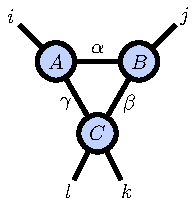
\includegraphics[scale=1]{figures/tikz/Tensor_Networks/basic_networks/basic_networks_c.pdf}}
	\subcaptionbox{\label{fig:basic_tensor_networks_matrix_vector_product}}
	{%
		\raisebox{\dimexpr.5\ht\largestimage-.5\height}
		{%
			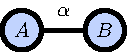
\includegraphics[scale=1]{figures/tikz/Tensor_Networks/basic_networks/basic_networks_a.pdf}
		}
	}
	\subcaptionbox{\label{fig:basic_tensor_networks_matrix_product}}
	{%
		\raisebox{\dimexpr.5\ht\largestimage-.5\height}
		{%
			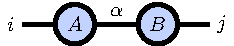
\includegraphics[scale=1]{figures/tikz/Tensor_Networks/basic_networks/basic_networks_b.pdf}
		}
	}
	\subcaptionbox{\label{fig:basic_tensor_networks_involved_contraction}}
	{%
		\usebox{\largestimage}
	}
	\caption{Tensor networks in diagrammatic notation. (a) Scalar product \eqref{eq:example_tensor_network_scalar_product}. (b) Matrix product \eqref{eq:example_tensor_network_matrix_product}. (c) More involved network consisting of three tensors \eqref{eq:example_tensor_network_involved_network}.}
	\label{fig:basic_tensor_network_diagrams}
\end{figure}
Because tensor contractions are linear, the order in which tensors are contracted does not change the result. However, the computational complexity does in general depend on the order of contractions and can thus be minimized by choosing the optimal contraction order. The computational complexity of a tensor contraction of two tensors is simply the product of all bond dimensions, where bond dimensions of contracted indices only appear in the product once. For example, the computational complexity of contracting tensors $B$ and $C$ from the contraction \eqref{eq:example_tensor_network_involved_network} scales as $\mathcal{O}(\chi_1\chi_2\chi_4\chi_5\chi_6\chi_7)$. \par
Given two normed vector spaces $V_1$ and $V_2$ with $\dim\left(V_1\right) = m$, $\dim\left(V_2\right) = n$, $m \le n$, an \textit{isometry} (sometimes also called \textit{semi-unitary}) is a linear, norm-preserving map $W: V_1 \rightarrow V_2$ from the smaller to the larger vector space. Each isometry can be represented by a $n\times m$ matrix $W$ fulfilling the \textit{isometry condition}
\begin{equation}
	\label{eq:isometry_condition_general}
	W^\dagger W = \id, \quad WW^\dagger = \mathbb{P},
\end{equation}
where $\mathbb{P} = \mathbb{P}^2$ is a projection. If $m = n$, it holds $\mathbb{P} = \id$ and $W$ is a \textit{unitary map}. An isometry tensor is a tensor that through grouping of indices and reshaping (i.e. matrixization) becomes an isometry. In tensor network diagrams, we draw isometries by decorating lines with arrows. Following the convention of \cite{cite:isometric_tensor_network_states_in_two_dimensions, cite:efficient_simulation_of_dynamics_in_two_dimensional_quantum_spin_systems}, we denote the indices belonging to the larger vector space by incoming arrows and the indices belonging to the smaller vector space by outgoing arrows. Unitary tensors are decorated with bidirectional arrows on all indices, where the grouping must be inferred from the context. Ordinary tensors are drawn without arrows. Tensor diagrams for isometric and unitary tensors are shown in Figure \figref{fig:isometries_and_unitaries_diagrams}.\par
\begin{figure}[ht]
	\centering
	\subcaptionbox{\label{fig:basic_isometries_isometric_matrix}}
	{%
		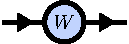
\includegraphics[scale=1]{figures/tikz/Tensor_Networks/basic_isometries/basic_isometries_a.pdf}
	}
	\par\bigskip
	\subcaptionbox{\label{fig:basic_isometries_unitary_matrix}}
	{%
	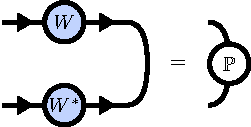
\includegraphics[scale=1]{figures/tikz/Tensor_Networks/basic_isometries/basic_isometries_c.pdf}
	}
	\par\bigskip
	\subcaptionbox{\label{fig:basic_isometries_isometric_tensor}}
	{%
		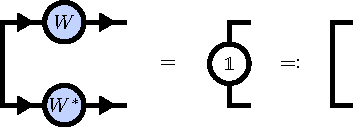
\includegraphics[scale=1]{figures/tikz/Tensor_Networks/basic_isometries/basic_isometries_b.pdf}
	}
	\caption{(a) An isometric matrix $W$ is depicted as a tensor diagram. The isometry condition \eqref{eq:isometry_condition_general} reduces contractions of $W$ with its adjoint to the identity matrix or to a projector $\mathbb{P}$. (b) A unitary matrix $U$ is drawn by using double arrows. For unitary matrices, the projector $\mathbb{P}$ is equal to the identity. (c) Isometric tensors of higher rank must fulfill the isometry condition by grouping of indices.}
	\label{fig:isometries_and_unitaries_diagrams}
\end{figure}
We lastly introduce an inner product for rank-$n$ tensors $A, B \in \mathbb{C}^{\chi_1\times\dots\times\chi_n}$, the \textit{Frobenius inner product}
\begin{equation}
	\label{eq:frobenius_inner_product}
	\left\langle A, B\right\rangle_\text{F} \coloneqq \sum_{\mu_1=1}^{\chi_1} \dots \sum_{\mu_n=1}^{\chi_n} A_{\mu_1,\dots,\mu_n}^*B_{\mu_1,\dots,\mu_n} = \Tr\left(A^\dagger B\right),
\end{equation}
where $A^*$ denotes the complex conjugate of $A$ and the last equality holds only if $n = 2$. The Frobenius inner product induces a norm, the \textit{Frobenius norm}
\begin{equation}
	\label{eq:frobenius_norm}
	\lVert A\rVert_\text{F} = \sqrt{\left\langle A, A\right\rangle_\text{F}},
\end{equation}
which can be used to define a measure of distance $\lVert A-B\rVert_\text{F}$ between two tensors $A$ and $B$.